% Supervisor briefing deck. Compile with pdflatex (Overleaf or MiKTeX):
%   pdflatex slides.tex
% Figures are generated by:  python presentations/supervisor/make_figures.py  (run from repo root)
%
% Structure
%   1  Title
%   2  The problem
%   3  Pipeline, built up over 4 clicks
%   4  What we found
%   5  Which numerical methods each pipeline stage uses
%   6  One fit, traced through our code (measured call counts)
%   7-9  Where each CSE 402 method runs: file, function, what it computes
%   10-15 Deep dives: safeguarded Newton, Levenberg-Marquardt, LU decomposition,
%         forward Euler, Heun, classical RK4
%   16 Summary
\documentclass[aspectratio=169,11pt]{beamer}

\usepackage[T1]{fontenc}
\usepackage{lmodern}
\usepackage{amsmath,amssymb}
\usepackage{booktabs}
\usepackage{graphicx}
\usepackage{listings}
\usepackage{microtype}
\usepackage{tikz}
\usetikzlibrary{arrows.meta,positioning,fit,backgrounds,calc,shadows.blur}

% ---- Theme: editorial research deck --------------------------------------
\definecolor{ink}{HTML}{142033}
\definecolor{navy}{HTML}{0A1930}
\definecolor{accent}{HTML}{147D92}
\definecolor{cyan}{HTML}{50C9CE}
\definecolor{hot}{HTML}{E26456}
\definecolor{good}{HTML}{28A879}
\definecolor{muted}{HTML}{607086}
\definecolor{soft}{HTML}{EAF4F5}
\definecolor{paper}{HTML}{F8FAFC}
\definecolor{line}{HTML}{D8E3EA}
\definecolor{gold}{HTML}{E8B44C}

\usetheme{default}
\setbeamertemplate{navigation symbols}{}
\setbeamersize{text margin left=0.62cm,text margin right=0.62cm}
\setbeamercolor{background canvas}{bg=paper}
\setbeamercolor{normal text}{fg=ink,bg=paper}
\setbeamercolor{frametitle}{fg=ink,bg=paper}
\setbeamercolor{title}{fg=white}
\setbeamercolor{subtitle}{fg=cyan}
\setbeamercolor{structure}{fg=accent}
\setbeamercolor{block title}{bg=accent,fg=white}
\setbeamercolor{block body}{bg=soft,fg=ink}
\setbeamerfont{title}{series=\bfseries,size=\fontsize{24}{27}}
\setbeamerfont{subtitle}{series=\mdseries,size=\large}
\setbeamerfont{frametitle}{series=\bfseries,size=\fontsize{16.5}{19}}
\setbeamerfont{block title}{series=\bfseries,size=\small}
\setbeamertemplate{itemize item}{\raise0.15ex\hbox{\color{accent}\scriptsize$\blacktriangleright$}}
\setbeamertemplate{itemize subitem}{\raise0.15ex\hbox{\color{cyan!70!accent}\tiny$\blacktriangleright$}}
\setbeamertemplate{enumerate item}{%
  \tikz[baseline=(n.base)]\node[fill=accent,text=white,font=\tiny\bfseries,
    circle,inner sep=1.1pt,minimum size=1.35em] (n) {\insertenumlabel};}
\setbeamertemplate{blocks}[rounded][shadow=false]
\setlength{\leftmargini}{1.25em}
\setlength{\leftmarginii}{1.1em}
\setlength{\tabcolsep}{4pt}
\renewcommand{\arraystretch}{1.14}

% A very light technical-grid texture: enough depth without competing with data.
\setbeamertemplate{background}{%
  \begin{tikzpicture}[remember picture,overlay]
    \fill[paper] (current page.south west) rectangle (current page.north east);
    \fill[soft!48] (current page.north east) -- ++(-2.8,0) -- ++(2.8,-2.8) -- cycle;
    \draw[line!55,line width=0.35pt] ($(current page.north east)+(-1.25,-0.35)$)
      circle[radius=0.62cm];
    \draw[cyan!14,line width=0.5pt] ($(current page.north east)+(-0.35,-1.25)$)
      circle[radius=0.86cm];
  \end{tikzpicture}}

% Title slide: high-contrast, asymmetric, and deliberately spare.
\setbeamertemplate{title page}{%
  
\begin{tikzpicture}[remember picture,overlay]
    \fill[navy] (current page.south west) rectangle (current page.north east);
    \fill[accent!30!navy] (current page.south west) -- ++(5.1,0) -- ++(-5.1,5.1) -- cycle;
    \fill[cyan!13!navy] (current page.north east) -- ++(-6.2,0) -- ++(6.2,-6.2) -- cycle;
    \draw[cyan!45,line width=1.1pt] ($(current page.north east)+(-1.4,-1.25)$) circle (0.78cm);
    \draw[cyan!18,line width=0.8pt] ($(current page.north east)+(-1.4,-1.25)$) circle (1.18cm);
    \fill[hot] ($(current page.north east)+(-1.4,-1.25)$) circle (2.2pt);
    \node[anchor=north west,text=cyan,font=\scriptsize\bfseries]
      at ($(current page.north west)+(0.82,-0.62)$) {CSE 402 \; / \; NUMERICAL ANALYSIS};
    \node[anchor=south east,text=white!12,font=\fontsize{54}{54}\selectfont\bfseries]
      at ($(current page.south east)+(-0.35,0.08)$) {SIR};
  \end{tikzpicture}%
  \vspace*{1.15cm}
  \begin{beamercolorbox}[wd=0.82\paperwidth,sep=0pt,left]{title}
    \usebeamerfont{title}\inserttitle\par
  \end{beamercolorbox}
  \vspace{0.32cm}
  {\color{cyan}\rule{1.15cm}{2.2pt}}\par
  \vspace{0.3cm}
  \begin{beamercolorbox}[wd=0.78\paperwidth,sep=0pt,left]{subtitle}
    \usebeamerfont{subtitle}\insertsubtitle\par
  \end{beamercolorbox}
  \vfill
  {\color{white}\small\bfseries\insertauthor\par}
  \vspace{0.18cm}
  {\color{white!62}\scriptsize\insertinstitute\par}
  \vspace*{0.58cm}
}

\setbeamertemplate{frametitle}{%
  \begin{beamercolorbox}[wd=\paperwidth,leftskip=0.62cm,rightskip=0.62cm,sep=0.10cm]{frametitle}
    \strut\usebeamerfont{frametitle}\insertframetitle
    \hfill\raisebox{0.15ex}{\color{accent}\scriptsize\bfseries\insertframenumber}
    \par\vspace{0.02cm}
    {\color{accent}\rule{1.05cm}{1.7pt}\color{line}\rule{\dimexpr\paperwidth-2.50cm\relax}{0.45pt}}
  \end{beamercolorbox}}
\setbeamertemplate{footline}{%
  \leavevmode
  \begin{beamercolorbox}[wd=\paperwidth,ht=0.34cm,dp=0.13cm,leftskip=0.62cm,rightskip=0.62cm]{normal text}
    {\color{muted}\tiny\bfseries CSE 402 \quad / \quad SECTION B, GROUP 2}
    \hfill
    {\color{muted}\tiny NUMERICAL ANALYSIS OF THE SIR MODEL \quad
      \textcolor{accent}{\insertframenumber/\inserttotalframenumber}}
  \end{beamercolorbox}%
  \begin{tikzpicture}[remember picture,overlay]
    \fill[line] (current page.south west) rectangle ++(\paperwidth,0.035cm);
    \fill[accent] (current page.south west) rectangle
      ++({\paperwidth*\insertframenumber/\inserttotalframenumber},0.035cm);
  \end{tikzpicture}}

\addtobeamertemplate{block begin}{\setlength{\textwidth}{\linewidth}}{}

\lstset{basicstyle=\ttfamily\scriptsize, columns=fullflexible, keepspaces=true,
        keywordstyle=\color{accent}\bfseries, commentstyle=\color{muted}, language=Python,
        frame=single, framerule=0.45pt, rulecolor=\color{line}, backgroundcolor=\color{soft!65},
        xleftmargin=4pt, xrightmargin=4pt, aboveskip=3pt, belowskip=3pt,
        showstringspaces=false}

\newcommand{\hl}[1]{\textcolor{accent}{\textbf{#1}}}
\newcommand{\deep}{\textcolor{hot}{$\bigstar$}}

% "Where exactly" bar for the deep-dive slides: #1 = code path, #2 = how often it runs
\newcommand{\where}[2]{%
  {\setlength{\fboxsep}{3pt}%
   \colorbox{soft}{\parbox{\dimexpr\linewidth-2\fboxsep\relax}{\tiny
     \textcolor{accent}{\textbf{In our code:}}~#1\\[1pt]
     \textcolor{accent}{\textbf{How often:}}~#2}}}\par\vspace{0.35em}}

% Section row inside the "where each method runs" tables
\newcommand{\labrow}[1]{\multicolumn{3}{@{}l}{\textcolor{accent}{\textbf{#1}}}\\[1pt]}

% ---- TikZ overlay helpers (show a node/arrow only on some clicks) ---------
\tikzset{
  invisible/.style={opacity=0, text opacity=0},
  visible on/.style={alt={#1{}{invisible}}},
  alt/.code args={<#1>#2#3}{\alt<#1>{\pgfkeysalso{#2}}{\pgfkeysalso{#3}}},
  box/.style={draw=line, fill=white, rounded corners=5pt, align=center,
              font=\small, minimum height=1.05cm, text width=3.0cm, line width=0.65pt,
              blur shadow={shadow blur steps=5,shadow xshift=0.35mm,shadow yshift=-0.35mm,
                           shadow opacity=12}},
  now/.style={draw=hot, fill=hot!6, line width=1.45pt},
  arr/.style={-{Stealth[length=2.2mm]}, semithick, color=accent!78!ink},
}

% ---- Pipeline locator strip for the deep-dive slides ----------------------
% #1 = index of the active stage (1 gold standard ... 6 evaluation)
\newcommand{\locator}[1]{%
  \begin{tikzpicture}[chip/.style={draw=line, rounded corners=3pt, font=\tiny,
      inner sep=1.5pt, minimum width=1.9cm, minimum height=0.36cm}]
    \foreach \name [count=\i] in {Gold standard,Synthetic data,Optimizer,ODE solver,Cost,Evaluation} {
      \ifnum\i=#1
        \node[chip, draw=accent, fill=accent, text=white, font=\tiny\bfseries] at (\i*2.05,0) {\name};
      \else
        \node[chip, fill=white, text=muted] at (\i*2.05,0) {\name};
      \fi
    }
  \end{tikzpicture}\par\vspace{0.15em}}

\title{Numerical Analysis of the SIR Epidemic Model}
\subtitle{Solver accuracy, parameter recovery, and robustness to noise}
\author{Saif Uz Zaman \and Sayaad Muzahid Masfi \and Ibtida bin Ahmed \and\\ Sakif Naieb Raiyan \and Aurchi Chowdhury}
\institute{CSE 402: Numerical Analysis, Simulation \& Modeling --- Section B, Group 2\\BUET}
\date{}

\begin{document}

% ===========================================================================
% PART 1: HIGH-LEVEL OVERVIEW
% ===========================================================================

% 1 -----------------------------------------------------------------------
{
\setbeamertemplate{background}{%
  
\begin{tikzpicture}[remember picture,overlay]
    \fill[navy] (current page.south west) rectangle (current page.north east);
    \fill[accent!30!navy] (current page.south west) -- ++(5.1,0) -- ++(-5.1,5.1) -- cycle;
    \fill[cyan!13!navy] (current page.north east) -- ++(-6.2,0) -- ++(6.2,-6.2) -- cycle;
  \end{tikzpicture}}
\begin{frame}[plain,t]
  \titlepage
\end{frame}
}

% 2 -----------------------------------------------------------------------
\begin{frame}[shrink=6]{The problem we study}
  \begin{columns}[T]
    \column{0.52\textwidth}
    \textbf{The SIR epidemic model} splits $N$ people into\\
    \textcolor{accent}{S}usceptible $\to$ \textcolor{hot}{I}nfectious $\to$ \textcolor{good}{R}ecovered:
    \[
      \dot S = -\tfrac{\beta S I}{N},\quad
      \dot I = \tfrac{\beta S I}{N} - \gamma I,\quad
      \dot R = \gamma I
    \]
    \vspace{-0.8em}
    \begin{itemize}\small
      \item $\beta$ = spreading rate, $\gamma$ = recovery rate, $R_0=\beta/\gamma$.
      \item In practice $\beta,\gamma$ are unknown: we \hl{fit} them to case counts by least squares.
      \item Each fit solves the ODE numerically, hundreds of times, and every solve is approximate.
      \item Our base paper (Capaldi et al., 2012) never varies the solver.
    \end{itemize}
    \vspace{0.2em}
    \begin{block}{Our question}
      \small How much does the \emph{solver} change the fitted $\beta,\gamma$, and when does that matter more than noise in the data?
    \end{block}
    \column{0.46\textwidth}
    \centering
    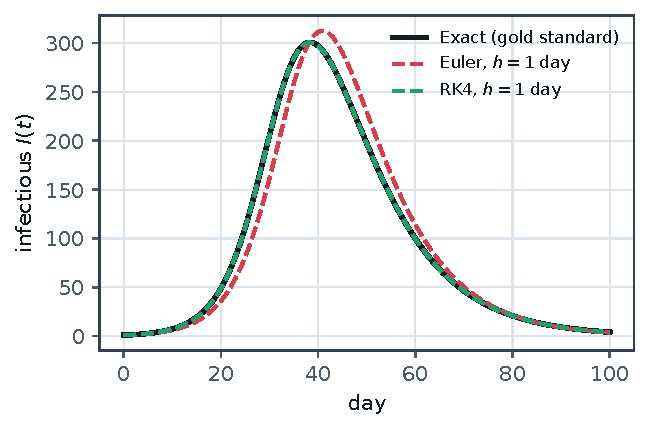
\includegraphics[width=\linewidth]{figures/epidemic_curve.pdf}\\[-0.2em]
    {\scriptsize\color{muted} Same $\beta,\gamma$, different solvers: Euler with 1-day steps draws a different curve.}
  \end{columns}
\end{frame}

% 3 -----------------------------------------------------------------------
\begin{frame}{Our pipeline}
  \centering
  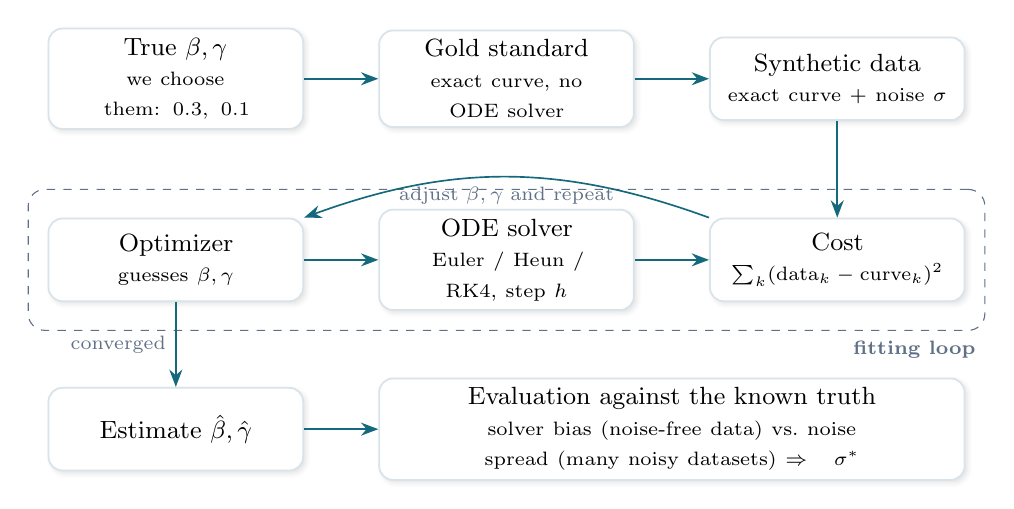
\begin{tikzpicture}
    % row 1: truth and data
    \node[box, alt=<1>{now}{}] (truth) at (0,0) {True $\beta,\gamma$\\{\scriptsize we choose them: $0.3,\ 0.1$}};
    \node[box, alt=<1>{now}{}] (gold) at (4.2,0) {Gold standard\\{\scriptsize exact curve, no ODE solver}};
    \node[box, visible on=<2->, alt=<2>{now}{}] (data) at (8.4,0) {Synthetic data\\{\scriptsize exact curve + noise $\sigma$}};
    % row 2: fitting loop
    \node[box, visible on=<3->, alt=<3>{now}{}] (opt) at (0,-2.3) {Optimizer\\{\scriptsize guesses $\beta,\gamma$}};
    \node[box, visible on=<3->, alt=<3>{now}{}] (solver) at (4.2,-2.3) {ODE solver\\{\scriptsize Euler / Heun / RK4, step $h$}};
    \node[box, visible on=<3->, alt=<3>{now}{}] (cost) at (8.4,-2.3) {Cost\\{\scriptsize $\sum_k(\mathrm{data}_k-\mathrm{curve}_k)^2$}};
    % row 3: output and evaluation
    \node[box, visible on=<4->, alt=<4>{now}{}] (est) at (0,-4.45) {Estimate $\hat\beta,\hat\gamma$};
    \node[box, visible on=<4->, alt=<4>{now}{}, text width=7.2cm] (eval) at (6.3,-4.45)
      {Evaluation against the known truth\\{\scriptsize solver bias (noise-free data) vs.\ noise spread (many noisy datasets) $\Rightarrow\ \sigma^*$}};

    \draw[arr] (truth) -- (gold);
    \draw[arr, visible on=<2->] (gold) -- (data);
    \draw[arr, visible on=<3->] (data) -- (cost);
    \draw[arr, visible on=<3->] (opt) -- (solver);
    \draw[arr, visible on=<3->] (solver) -- (cost);
    \draw[arr, visible on=<3->] (cost.north west) to[out=160, in=20]
      node[below, font=\scriptsize, color=muted, pos=0.5]{adjust $\beta,\gamma$ and repeat} (opt.north east);
    \draw[arr, visible on=<4->] (opt) -- node[left, font=\scriptsize, color=muted]{converged} (est);
    \draw[arr, visible on=<4->] (est) -- (eval);

    \begin{scope}[on background layer]
      \node[fit=(opt)(solver)(cost), draw=muted, dashed, rounded corners=6pt,
            inner sep=7pt, visible on=<3->] (loop) {};
    \end{scope}
    \node[font=\scriptsize\bfseries, color=muted, anchor=north east, visible on=<3->]
      at (loop.south east) {fitting loop};
  \end{tikzpicture}

  \vspace{0.3em}
  \small
  \only<1>{\textbf{Step 1.} We pick the true $\beta,\gamma$ ourselves and compute the \emph{exact} epidemic curve with a method that uses no ODE solver. This is our answer key.}%
  \only<2>{\textbf{Step 2.} We read the exact curve on the observation days and add random noise of controlled size $\sigma$. This imitates real, messy case counts.}%
  \only<3>{\textbf{Step 3.} The standard fitting loop: guess $\beta,\gamma$, let the solver draw the curve, score it against the data, adjust, repeat. \textcolor{hot}{The solver is our experimental variable.}}%
  \only<4>{\textbf{Step 4.} Because we know the truth, we can split the error in $\hat\beta,\hat\gamma$ into \emph{solver bias} and \emph{noise spread}, and find the noise level $\sigma^*$ where they are equal.}
\end{frame}

% 4 -----------------------------------------------------------------------
\begin{frame}{What we found}
  \begin{columns}[T]
    \column{0.49\textwidth}
    \centering
    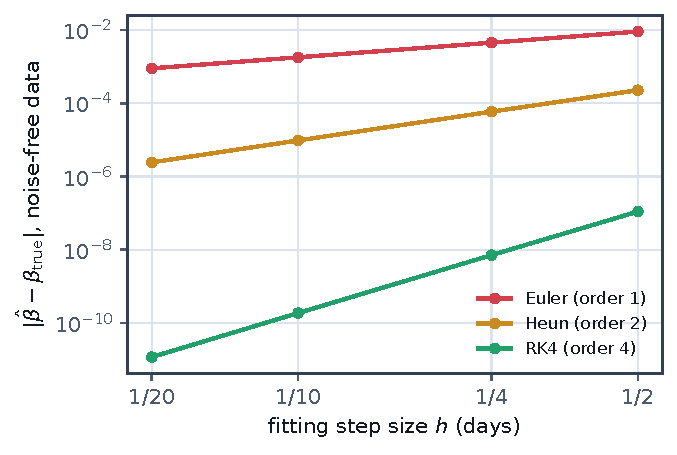
\includegraphics[width=\linewidth,height=3.25cm,keepaspectratio]{figures/bias_vs_h.pdf}\\[-0.1em]
    \small\textbf{1. Solver error becomes parameter bias.}\\
    {\scriptsize On perfect data, the error in $\hat\beta$ shrinks with the solver's own order: Euler 1, Heun 2, RK4 4 (E07).}
    \column{0.49\textwidth}
    \centering
    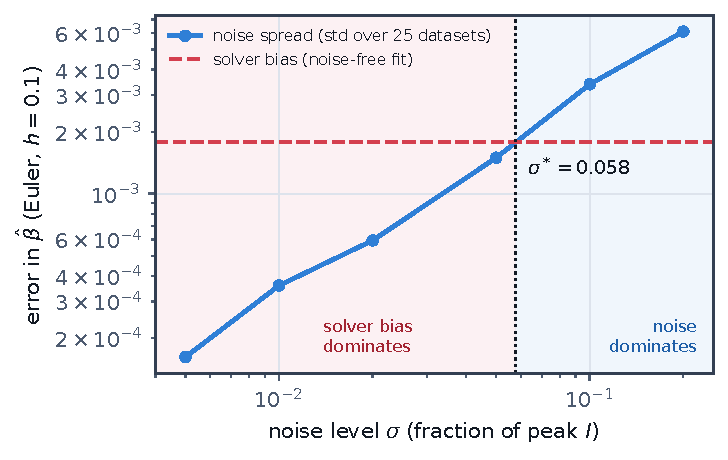
\includegraphics[width=\linewidth,height=3.25cm,keepaspectratio]{figures/crossover.pdf}\\[-0.1em]
    \small\textbf{2. There is a crossover noise level $\sigma^*$.}\\
    {\scriptsize Euler, $h=0.1$: below $\sigma^*=0.058$ the solver dominates the error; above it, noise does (E13).}
  \end{columns}
  \vspace{0.4em}
  \begin{center}\small
    Also (E01): observed orders $\hat p$ = 1.03 (Euler), 1.94 (Heun), 3.94 (RK4), 0.97 (backward Euler), 2.00 (trapezoidal).
  \end{center}
\end{frame}

% ===========================================================================
% PART 2: NUMERICAL METHODS
% ===========================================================================

% 5 -----------------------------------------------------------------------
\begin{frame}{Which numerical methods each pipeline stage uses}
  \centering
  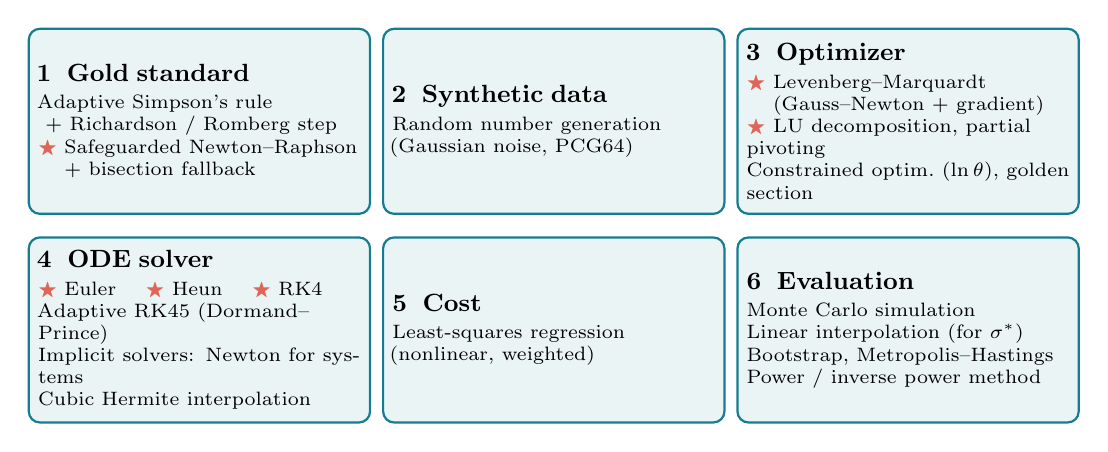
\begin{tikzpicture}[
      card/.style={draw=accent, fill=soft, rounded corners=4pt, align=left,
                   text width=4.1cm, minimum height=2.35cm, font=\scriptsize, anchor=north,
                   line width=0.8pt},
      head/.style={font=\small\bfseries, color=ink}]
    \node[card] (c1) at (0,0)    {{\small\bfseries 1\; Gold standard}\\[2pt]
      Adaptive Simpson's rule\\ \ + Richardson / Romberg step\\
      \deep\ Safeguarded Newton--Raphson\\ \phantom{\deep}\ + bisection fallback};
    \node[card] (c2) at (4.5,0) {{\small\bfseries 2\; Synthetic data}\\[2pt]
      Random number generation\\ (Gaussian noise, PCG64)};
    \node[card] (c3) at (9.0,0)  {{\small\bfseries 3\; Optimizer}\\[2pt]
      \deep\ Levenberg--Marquardt\\ \phantom{\deep}\ (Gauss--Newton + gradient)\\
      \deep\ LU decomposition, partial pivoting\\
      Constrained optim.\ ($\ln\theta$), golden section};
    \node[card] (c4) at (0,-2.65)    {{\small\bfseries 4\; ODE solver}\\[2pt]
      \deep\ Euler \quad \deep\ Heun \quad \deep\ RK4\\ Adaptive RK45 (Dormand--Prince)\\
      Implicit solvers: Newton for systems\\
      Cubic Hermite interpolation};
    \node[card] (c5) at (4.5,-2.65) {{\small\bfseries 5\; Cost}\\[2pt]
      Least-squares regression\\ (nonlinear, weighted)};
    \node[card] (c6) at (9.0,-2.65)  {{\small\bfseries 6\; Evaluation}\\[2pt]
      Monte Carlo simulation\\
      Linear interpolation (for $\sigma^*$)\\
      Bootstrap, Metropolis--Hastings\\
      Power / inverse power method};
  \end{tikzpicture}

  \vspace{0.4em}
  {\small \deep\ = explained in detail on the following slides.}
\end{frame}

% 6 -----------------------------------------------------------------------
\begin{frame}[shrink=4]{One fit, traced through our code}
  {\small One E13 fit: Euler, $h=0.1$, noise $\sigma=0.05$, 60 daily counts. Calls counted by instrumenting the code.}

  \vspace{0.4em}
  \scriptsize
  \begin{tabular}{@{}p{2.25cm}p{5.0cm}p{5.0cm}r@{}}
    \toprule
    Stage & Code that runs & Numerical method & Calls\\
    \midrule
    \textbf{1 Gold standard} & \texttt{SIRReference.s\_infinity} & Safeguarded Newton: final size (sets the table's range) & 1\\
     & \texttt{\_ensure\_table} $\to$ \texttt{adaptive\_simpson} & Adaptive Simpson on 2{,}000 cells of $t(R)$ & 2{,}000\\
     & \texttt{trajectory} $\to$ \texttt{r\_of\_t} $\to$ \texttt{newton\_safe} & Safeguarded Newton: $R$ on each day (plus 333 short Simpson integrals) & 60\\
    \textbf{2 Synthetic data} & \texttt{rng.normal}, \texttt{rng.uniform} & Gaussian noise; random start $\theta_0$ & 62 draws\\
    \textbf{3 Optimizer} & \texttt{levenberg\_marquardt} & Levenberg--Marquardt rounds & 5\\
     & \texttt{lu\_factor}, \texttt{lu\_solve} & LU: step $\delta$ each round, then Cov$(\hat\theta)$ & 6\\
    \textbf{4 ODE solver} & \texttt{integrate(model, y0, $\theta$, span, solver, h)} & Runge--Kutta solve of SIR & 11\\
     & \texttt{integrate\_with\_sensitivities} & Same solver on 9 variables $[y,\ \partial y/\partial\beta,\ \partial y/\partial\gamma]$ & 5\\
     & \texttt{SolveResult.at(t\_obs)} & Cubic Hermite interpolation onto the 60 days & every solve\\
    \textbf{5 Cost} & \texttt{ForwardModel.residuals}, \texttt{.cost} & Least squares $\tfrac12\sum_k r_k^2$ & 11\\
    \textbf{6 Evaluation} & \texttt{E13\_crossover.run} & Monte Carlo: repeat this whole fit; linear interpolation for $\sigma^*$ & 459 fits\\
    \bottomrule
  \end{tabular}

  \vspace{0.5em}
  {\scriptsize\color{muted} 459 = 3 step sizes $\times$ (3 noise-free bias fits + 6 noise levels $\times$ 25 datasets), quick profile. That is about 7{,}300 ODE solves for one experiment.}
\end{frame}

% 7 -----------------------------------------------------------------------
\begin{frame}[shrink=4]{Where each CSE 402 method runs (1/3): Labs 1 and 2}
  \scriptsize
  \begin{tabular}{@{}p{3.1cm}p{5.6cm}p{5.4cm}@{}}
    \toprule
    Method & Where in our code & What it computes\\
    \midrule
    \labrow{Lab 1: approximations, errors, root finding}
    Truncation, round-off error & \texttt{diagnostics.py}: \texttt{observed\_order}, \texttt{mass\_error}, \texttt{phase\_invariant\_drift} & Order $\hat p$ against the gold standard (E01); $S+I+R$ stuck at round-off (E02); bias $\propto h^p$ (E07)\\
    \deep\ Newton--Raphson + bisection & \texttt{roots/newton.py: newton\_safe}, called by \texttt{reference.py: r\_of\_t, s\_infinity} & $R$ on every observation day; final size $S_\infty$\\
    Newton for systems & \texttt{solvers/implicit.py: \_newton\_solve\_stage} & $y_{n+1}$ of each backward-Euler / trapezoidal step (E01, E03)\\[2pt]
    \labrow{Lab 2: linear systems and eigenvalues}
    \deep\ LU, partial pivoting & \texttt{linalg/lu.py}, called by \texttt{lm.py}, \texttt{gaussnewton.py}, \texttt{implicit.py}, \texttt{eigen.py} & LM step $\delta$; implicit Newton steps; Cov$(\hat\theta)=\hat\sigma^2(J^\top J)^{-1}$\\
    Condition number & \texttt{lu.py: cond\_estimate}; \texttt{eigen.py: cond2} & $\kappa(J^\top J)$ of the cost valley (E05); $\kappa_2$ with $I_0$ unknown (E10)\\
    Power method & \texttt{eigen.py: spectral\_radius}, via \texttt{diagnostics.stability\_metric} & $h\,\rho(J_y f)$ stability map (E03)\\
    Inverse power, Hotelling deflation & \texttt{eigen.py: inverse\_power\_method}, \texttt{symmetric\_eigen} & $\lambda_{\min}$ for $\kappa_2$ (E10); ellipse axes (E11, E14); valley direction (E05)\\
    \bottomrule
  \end{tabular}
\end{frame}

% 8 -----------------------------------------------------------------------
\begin{frame}[shrink=4]{Where each CSE 402 method runs (2/3): Lab 3 and Home Assignment 1}
  \scriptsize
  \begin{tabular}{@{}p{3.1cm}p{5.6cm}p{5.4cm}@{}}
    \toprule
    Method & Where in our code & What it computes\\
    \midrule
    \labrow{Lab 3: random numbers and Monte Carlo}
    Random number generation & \texttt{np.random.default\_rng(seed)} in every stochastic experiment (NumPy's PCG64, not our own) & Noise (\texttt{rng.normal}), random starts (\texttt{rng.uniform}), resampling (\texttt{rng.integers})\\
    Monte Carlo & Replicate loops in E07--E10, E13; \texttt{uq/montecarlo.py} & Bias, spread and RMSE of $\hat\beta,\hat\gamma$; UQ route 3 (E11)\\
    Bootstrap & \texttt{uq/bootstrap.py: residual\_bootstrap}; RMSE band in E08 & Uncertainty cloud (E11); CI on the RMSE curve (E08)\\
    Metropolis--Hastings & \texttt{uq/mcmc.py: run\_mcmc}, 4 chains & Posterior of $\beta,\gamma$ with $\hat R$ and ESS (E11)\\[2pt]
    \labrow{Home Assignment 1: QR and optimization}
    \deep\ Gradient methods (LM) & \texttt{estimate/lm.py: levenberg\_marquardt} & The fit in E06--E11, E13, E14, bootstrap and Monte Carlo\\
    Newton's method (Gauss--Newton) & \texttt{estimate/gaussnewton.py: gauss\_newton} & Optimizer comparison (E06)\\
    Golden-section search & \texttt{estimate/golden.py}; \texttt{uq/profile.py} & Coordinate descent (E06); profile likelihood (E11)\\
    Constrained optimization & $u=\ln\theta$ in \texttt{lm.py}; box bounds in \texttt{golden.py} & Keeps $\beta,\gamma>0$\\
    QR (Householder) & \texttt{linalg/qr.py}; option \texttt{use\_qr} in \texttt{gaussnewton.py} & Implemented and tested; reported fits use LU\\
    \bottomrule
  \end{tabular}
\end{frame}

% 9 -----------------------------------------------------------------------
\begin{frame}[shrink=4]{Where each CSE 402 method runs (3/3): Lab 4 and ODE solvers}
  \scriptsize
  \begin{tabular}{@{}p{3.1cm}p{5.6cm}p{5.4cm}@{}}
    \toprule
    Method & Where in our code & What it computes\\
    \midrule
    \labrow{Lab 4: curve fitting, interpolation, integration}
    Least-squares regression & \texttt{ForwardModel.cost}; \texttt{diagnostics.observed\_order} & Every fit's objective; slope of $\log e$ vs.\ $\log h$ gives $\hat p$ (E01)\\
    Linear interpolation & \texttt{E13\_crossover.run} & $\sigma^*$ between two tested noise levels\\
    Cubic Hermite spline & \texttt{solvers/base.py: SolveResult.at} & Curve and sensitivities on the observation days\\
    Simpson, Richardson/Romberg & \texttt{quadrature/adaptive.py: adaptive\_simpson}, called by \texttt{reference.py} & Gold-standard integral $t(R)$\\
    Composite Simpson, trapezoid & \texttt{quadrature/simpson.py}, used by \texttt{observe.incidence} & Incidence observations: tested, not in reported runs\\
    Numerical differentiation & \texttt{np.gradient} in \texttt{SolveResult.at}; complex step in \texttt{tests/test\_models.py} & Hermite node slopes; checks of our analytic Jacobians\\[2pt]
    \labrow{Course textbook, Part 7: ODEs}
    \deep\ Euler, Heun, RK4; RK45 & \texttt{solvers/explicit.py}, \texttt{rk45.py}, all through \texttt{solvers.integrate} & Every curve the optimizer sees; RK45 reference for SEIR/SIRS (E12)\\
    Implicit Euler, trapezoidal & \texttt{solvers/implicit.py} & Stability contrast (E01, E03)\\
    \bottomrule
  \end{tabular}

  \vspace{0.4em}
  {\scriptsize\color{muted} All methods are hand-written in \texttt{core/sirlab}; SciPy appears only in tests, as a cross-check. Not used: false position, Bairstow, Gauss--Jordan, divided differences.}
\end{frame}

% 10 ----------------------------------------------------------------------
\begin{frame}[shrink=5]{Deep dive 1: safeguarded Newton--Raphson}
  \locator{1}
  \where{\texttt{SIRReference.trajectory(t\_obs)} $\to$ \texttt{r\_of\_t(t)} $\to$ binary search for the table cell $\to$ \texttt{newton\_safe(f, f', $\rho_{lo}$, $\rho_{hi}$)}; and \texttt{s\_infinity} $\to$ \texttt{newton\_safe(g, g', $10^{-9}N$, $S_0$)} (\texttt{roots/newton.py}).}
        {Once per observation day (60 per dataset in E07 and E13), plus once for $S_\infty$ per $(\beta,\gamma)$.}
  \begin{columns}[T]
    \column{0.5\textwidth}
    \small
    \textbf{Where:} the integral gives day $t$ for a given $R$. We need the reverse: \emph{which $R$ on day $t$?} Solve
    \[ f(R) = t(R) - t^* = 0, \qquad f'(R) = \frac{1}{\gamma\, I(R)} \]
    The derivative is known exactly: it is the integrand itself.

    \vspace{0.2em}
    \textbf{Newton:} $R_{k+1} = R_k - f(R_k)/f'(R_k)$. Finding $R$ on day 30:

    \vspace{0.1em}
    \scriptsize
    \begin{tabular}{@{}clr@{}}
      \toprule
      $k$ & $R_k$ & $t(R_k)-30$\\
      \midrule
      0 & 300 & $+6.15$\\
      1 & 119.33 & $-1.17$\\
      2 & 140.75 & $-0.067$\\
      3 & 142.1212 & $-2.2\times10^{-4}$\\
      4 & 142.12560253 & $-2.2\times10^{-9}$\\
      \bottomrule
    \end{tabular}
    \quad {\color{muted} digits roughly double each step}
    \column{0.48\textwidth}
    \small
    \textbf{The danger:} plain Newton can converge to a meaningless root. On the final-size equation $\ln(S_0/S_\infty) = R_0 (N-S_\infty)/N$, starting from 500 it converges to \textcolor{hot}{$S_\infty = 1000.5$}: more healthy people than the village has.

    \vspace{0.3em}
    \textbf{Safeguard} (\texttt{roots/newton.py}, \texttt{newton\_safe}):
    \begin{itemize}\scriptsize
      \item Keep a bracket $[lo, hi]$ where $f$ changes sign.
      \item Take the Newton step only if it stays inside the bracket and at least halves it; otherwise \hl{bisect}.
      \item Newton's speed when safe, bisection's guarantee otherwise.
    \end{itemize}
    \textbf{Used for:} every exact data point (inverting $t(R)$) and the final size $S_\infty = 59.448$.
  \end{columns}
\end{frame}

% 11 ----------------------------------------------------------------------
\begin{frame}[shrink=3]{Deep dive 2: Levenberg--Marquardt}
  \locator{3}
  \where{E06--E11, E13, E14, \texttt{uq/bootstrap.py}, \texttt{uq/montecarlo.py} $\to$ \texttt{levenberg\_marquardt(fwd, obs, $\theta_0$)}. Each round: \texttt{fwd.residuals} (1 ODE solve) + \texttt{fwd.jacobian} $\to$ \texttt{integrate\_with\_sensitivities} + a trial \texttt{fwd.cost} (\texttt{estimate/lm.py}).}
        {Once per fit. The traced E13 fit took 5 rounds and 16 ODE solves; E13 alone runs 459 fits.}
  \begin{columns}[T]
    \column{0.52\textwidth}
    \small
    \textbf{Problem:} minimise $\tfrac12\sum_k r_k(\theta)^2$, with residuals $r$ = curve $-$ data and $\theta = (\beta,\gamma)$.

    \vspace{0.2em}
    \textbf{Each round} solve for the step $\delta$:
    \[ \big(J^\top J + \lambda\,\mathrm{diag}(J^\top J)\big)\,\delta = -J^\top r \]
    \vspace{-1.1em}
    \begin{itemize}\scriptsize
      \item $\lambda\to0$: Gauss--Newton (fast near the minimum).
      \item $\lambda$ large: scaled gradient descent (safe far away).
      \item Step rejected: $\lambda\times10$. Step accepted: $\lambda\div10$.
      \item $J=\partial r/\partial\theta$ comes from sensitivity equations integrated \emph{by the same solver}, not from finite differences.
      \item We optimise $u=\ln\theta$, so $\beta,\gamma$ stay positive (constrained optimization).
    \end{itemize}
    \column{0.46\textwidth}
    \scriptsize
    \textbf{Real run} (12 counts, 5\% noise, RK4):

    \vspace{0.2em}
    \begin{tabular}{@{}crrr@{}}
      \toprule
      Round & $\beta$ & $\gamma$ & Cost\\
      \midrule
      0 & 0.2500 & 0.1200 & 134\,396\\
      1 & 0.3781 & 0.1615 & 82\,360\\
      2 & 0.2770 & 0.0983 & 14\,067\\
      3 & 0.3009 & 0.1022 & 1\,241\\
      4 & 0.2977 & 0.0996 & 978.4\\
      8 & 0.2978 & 0.0996 & 978.1\\
      \bottomrule
    \end{tabular}

    \vspace{0.4em}
    \textbf{Cost:} 17 solver runs, against 103 for Nelder--Mead on the same data. In E06, LM succeeded 100\% of the time (mean 8.5 rounds), so it is the estimator in every main experiment (\texttt{estimate/lm.py}).
  \end{columns}
\end{frame}

% 12 ----------------------------------------------------------------------
\begin{frame}[shrink=5]{Deep dive 3: LU decomposition with partial pivoting}
  \locator{3}
  \where{\texttt{levenberg\_marquardt} $\to$ \texttt{lu\_factor($J^\top J + \lambda\,\mathrm{diag} + 10^{-14}I$)}, \texttt{lu\_solve($-J^\top r$)}; at the end \texttt{lu\_solve($J^\top J$, $I$)} for Cov$(\hat\theta)$. Also \texttt{implicit.py: \_newton\_solve\_stage} and \texttt{eigen.py: inverse\_power\_method} (\texttt{linalg/lu.py}).}
        {Every LM round (6 factorizations in the traced fit), every implicit-solver Newton iteration, and once per inverse-power run.}
  \begin{columns}[T]
    \column{0.48\textwidth}
    \small
    \textbf{Method} (Doolittle, \texttt{linalg/lu.py}): factor $PA = LU$.
    \begin{enumerate}\scriptsize
      \item For each column, choose the largest $|a_{ik}|$ as pivot and swap rows (limits round-off growth).
      \item Eliminate below the pivot; store each multiplier $\ell_{ik}$ in the freed lower slot.
      \item Solve $Ly = Pb$ (forward), then $Ux = y$ (back).
    \end{enumerate}
    \vspace{0.2em}
    \textbf{Used in:}
    \begin{itemize}\scriptsize
      \item every LM / Gauss--Newton round ($2\times2$ or $3\times3$),
      \item every implicit-solver Newton step, $(I-hJ)\,\delta = -G$,
      \item the inverse power method (factor once, solve many times),
      \item the covariance $(J^\top J)^{-1}$ for the confidence ellipse.
    \end{itemize}
    {\scriptsize Tested against \texttt{scipy.linalg.lu\_factor} to $10^{-12}$.}
    \column{0.5\textwidth}
    \scriptsize
    \textbf{Example: LM round 1 from the previous slide}
    \[
      \underbrace{\begin{pmatrix} 1\,662\,008 & -1\,001\,469\\ -1\,001\,469 & 712\,563 \end{pmatrix}}_{J^\top J + \lambda\,\mathrm{diag}}
      \delta =
      \begin{pmatrix} 390\,138\\ -202\,664 \end{pmatrix}
    \]
    \begin{itemize}\scriptsize
      \item Pivot: $|1\,662\,008| > |{-1\,001\,469}|$, so no swap.
      \item $\ell_{21} = -1\,001\,469 / 1\,662\,008 = -0.6026$
      \item $u_{22} = 712\,563 - (-0.6026)(-1\,001\,469) = 109\,112$
      \item Forward: $y = (390\,138,\ 32\,420)$
      \item Back: $\delta_2 = 32\,420/109\,112 = 0.2971$,\\
            $\delta_1 = (390\,138 + 1\,001\,469\,\delta_2)/1\,662\,008 = 0.4138$
      \item New $\theta = \theta\,e^{\delta} = (0.25\,e^{0.4138},\ 0.12\,e^{0.2971}) = \mathbf{(0.3781,\ 0.1615)}$
    \end{itemize}
    {\color{muted} Exactly round 1 of the LM table.}
  \end{columns}
\end{frame}

% 13 ----------------------------------------------------------------------
\begin{frame}[fragile,shrink=5]{Deep dive 4: forward Euler}
  \locator{4}
  \where{\texttt{solvers.integrate(\ldots, solver="euler", h)} $\to$ \texttt{solvers/explicit.py: integrate\_euler}, called from \texttt{ForwardModel.predict} and \texttt{integrate\_with\_sensitivities} inside every fit.}
        {The fitting solver for all 459 fits of E13 (about 7{,}300 solves) and the Euler cells of E07; swept over the step-size ladder in E01--E04 and E12; compared with RK4 on the Eyam data (E14).}
  \begin{columns}[T]
    \column{0.5\textwidth}
    \small
    \textbf{Idea:} use the slope at the start of the step for the whole step.
    \[ y_{n+1} = y_n + h\, f(t_n, y_n) \]
    \vspace{-0.9em}

    {\scriptsize This is the Taylor series $y(t+h) = y + h y' + \tfrac{h^2}{2} y'' + \cdots$ cut after the $h$ term. Local error $\approx \tfrac{h^2}{2}y''$, global error $O(h)$: \hl{order 1}, one $f$ evaluation per step.}

    \vspace{0.3em}
    \textbf{Code} (\texttt{solvers/explicit.py}):
\begin{lstlisting}[basicstyle=\ttfamily\tiny]
f = model.rhs(t[k], yk, theta)
n_fev += 1
y[k + 1] = yk + h * f
if np.any(y[k + 1] < 0):
    negativity_events += 1
\end{lstlisting}
    {\scriptsize The loop also flags negative compartments and blow-up; E03 uses these flags for the stability map.}
    \column{0.48\textwidth}
    \scriptsize
    \textbf{One step} from $(S,I,R)=(990,10,0)$, $h=1$: slope $(-2.97,\ 1.97,\ 1.00)$ gives $I(1)=11.97$ (exact 12.17165). The error, $-0.20$, is predicted by the dropped term $\tfrac{h^2}{2}I''\approx 0.19$.

    \vspace{0.3em}
    \begin{tabular}{@{}lccc@{}}
      \toprule
      $h$ & 1 & 0.1 & 0.01\\
      \midrule
      Error in $I$ at day 30 & 44.3 & 4.46 & 0.444\\
      \bottomrule
    \end{tabular}\\[2pt]
    $10\times$ smaller $h$ $\Rightarrow$ $10\times$ smaller error. Measured order 1.03 (E01).

    \vspace{0.3em}
    \textbf{Effect on the fit:} on perfect data with $h=1$, $\hat\beta = 0.3178$ instead of 0.3 (\hl{6\% high}). In E13, $\sigma^* = 0.058$ at $h=0.1$ and 0.156 at $h=0.25$.

    \vspace{0.3em}
    \textbf{Stability:} on $y'=\lambda y$ each step multiplies by $1+h\lambda$, so real $\lambda<0$ needs $h|\lambda|\le 2$.

    \vspace{0.3em}
    {\color{muted} $S+I+R$ stays at 1000 to round-off even when $I$ is 44 people wrong (E02).}
  \end{columns}
\end{frame}

% 14 ----------------------------------------------------------------------
\begin{frame}[fragile,shrink=5]{Deep dive 5: Heun's method}
  \locator{4}
  \where{\texttt{solvers.integrate(\ldots, solver="heun", h)} $\to$ \texttt{solvers/explicit.py: integrate\_heun}; same call sites as Euler.}
        {The Heun cells of E07 (bias vs.\ $h$), the step-size ladders of E01--E04, and the model variants in E12.}
  \begin{columns}[T]
    \column{0.5\textwidth}
    \small
    \textbf{Idea:} predict with Euler, then correct with the average of the slopes at both ends: the trapezoidal rule applied to the ODE.
    \[ \tilde y = y_n + h f(t_n,y_n), \quad y_{n+1} = y_n + \tfrac h2\big[f(t_n,y_n) + f(t_{n+1},\tilde y)\big] \]
    \vspace{-0.9em}

    {\scriptsize Matches the Taylor series through the $h^2$ term. Local error $O(h^3)$, global $O(h^2)$: \hl{order 2}, two $f$ evaluations per step.}

    \vspace{0.3em}
    \textbf{Code} (\texttt{solvers/explicit.py}):
\begin{lstlisting}[basicstyle=\ttfamily\tiny]
f0 = model.rhs(t[k], yk, theta)
y_pred = yk + h * f0
f1 = model.rhs(t[k + 1], y_pred, theta)
n_fev += 2
y[k + 1] = yk + (h / 2.0) * (f0 + f1)
\end{lstlisting}
    \column{0.48\textwidth}
    \scriptsize
    \textbf{One step} from $(990,10,0)$, $h=1$:

    \vspace{0.1em}
    \begin{tabular}{@{}lccc@{}}
      \toprule
      & $S$ & $I$ & $R$\\
      \midrule
      $k_1$ (slope at start) & $-2.97$ & $1.97$ & $1.00$\\
      trial $\tilde y = y_n + h k_1$ & 987.03 & 11.97 & 1.00\\
      $k_2$ (slope at trial point) & $-3.54$ & $2.35$ & $1.20$\\
      $y_{n+1}$ & 986.74 & \textbf{12.159} & 1.10\\
      \bottomrule
    \end{tabular}\\[2pt]
    Error in $I$: $-0.013$, about 15$\times$ smaller than Euler's.

    \vspace{0.3em}
    \begin{tabular}{@{}lccc@{}}
      \toprule
      $h$ & 1 & 0.1 & 0.01\\
      \midrule
      Error in $I$ at day 30 & 2.57 & 0.0289 & 0.00029\\
      \bottomrule
    \end{tabular}\\[2pt]
    $10\times$ smaller $h$ $\Rightarrow$ about $100\times$ smaller error. Measured order 1.94 (E01).

    \vspace{0.3em}
    \textbf{Effect on the fit (E07):} bias in $\hat\beta$ falls from $5.88\times10^{-5}$ ($h=0.25$) to $2.43\times10^{-6}$ ($h=0.05$), a factor of 24.2 (theory $5^2=25$).

    \vspace{0.3em}
    \textbf{Stability:} factor $1+z+\tfrac{z^2}{2}$ with $z=h\lambda$; same real-axis limit as Euler ($h|\lambda|\le2$). Heun buys accuracy, not stability.
  \end{columns}
\end{frame}

% 15 ----------------------------------------------------------------------
\begin{frame}[fragile,shrink=5]{Deep dive 6: classical RK4}
  \locator{4}
  \where{\texttt{solvers.integrate(\ldots, solver="rk4", h)} $\to$ \texttt{solvers/explicit.py: integrate\_rk4}; then \texttt{SolveResult.at(t\_obs)} (cubic Hermite) $\to$ \texttt{prevalence}. The Jacobian uses the same \texttt{integrate} on the 9-variable system $[y,\ \partial y/\partial\beta,\ \partial y/\partial\gamma]$.}
        {The default fitting solver: E05, E06 and E08--E11 fit with RK4, and E05, E06, E11 also generate their data with RK4 at $h=0.1$. Also the RK4 cells of E07, E01--E04, E12, and the Eyam fit (E14).}
  \begin{columns}[T]
    \column{0.5\textwidth}
    \small
    \textbf{Idea:} sample the slope four times inside the step (start, middle twice, end) and move by a weighted average.

    \vspace{0.2em}
    \textbf{Code} (\texttt{solvers/explicit.py}):
\begin{lstlisting}[basicstyle=\ttfamily\tiny]
k1 = model.rhs(tk,         yk,              theta)
k2 = model.rhs(tk + h/2.0, yk + (h/2.0)*k1, theta)
k3 = model.rhs(tk + h/2.0, yk + (h/2.0)*k2, theta)
k4 = model.rhs(tk + h,     yk + h*k3,       theta)
y[k+1] = yk + (h/6.0)*(k1 + 2.0*k2 + 2.0*k3 + k4)
\end{lstlisting}
    \scriptsize Weights 1, 2, 2, 1: Simpson's 1, 4, 1 with the middle split in two. Matches Taylor through $h^4$: \hl{order 4}, four $f$ evaluations per step.

    \vspace{0.2em}
    \textbf{One step} from $I=10$, $h=1$: slopes $1.970,\ 2.159,\ 2.177,\ 2.387$ give $I(1) = 12.17162$ (exact 12.17165). Error $-0.00003$, about 7{,}000$\times$ smaller than Euler's.
    \column{0.48\textwidth}
    \scriptsize
    \begin{tabular}{@{}lccc@{}}
      \toprule
      $h$ & 1 & 0.1 & 0.01\\
      \midrule
      Error in $I$ at day 30 & 0.0045 & $5.1\times10^{-7}$ & $5.0\times10^{-11}$\\
      \bottomrule
    \end{tabular}\\[2pt]
    $10\times$ smaller $h$ $\Rightarrow$ about $10{,}000\times$ smaller error. Measured order 3.94 (E01). Below $h\approx0.001$ round-off takes over.

    \vspace{0.3em}
    \textbf{Same work} (120 $f$ evaluations to day 30): Euler error 11.2, Heun 0.68, \textbf{RK4 0.0045}.

    \vspace{0.3em}
    \textbf{Effect on the fit (E07):} bias in $\hat\beta$ falls from $7.17\times10^{-9}$ ($h=0.25$) to $1.18\times10^{-11}$ ($h=0.05$), a factor of 606 (theory $5^4=625$).

    \vspace{0.3em}
    \textbf{Stability:} real-axis limit $h|\lambda|\le 2.79$.

    \vspace{0.3em}
    {\color{muted} Adaptive RK45 (Dormand--Prince) builds on the same idea and chooses $h$ itself; it is the reference for SEIR/SIRS (E12). The TypeScript copy repeats these lines in the same order, so both agree to about $10^{-12}$.}
  \end{columns}
\end{frame}

% 16 ----------------------------------------------------------------------
\begin{frame}{Summary}
  \begin{columns}[T]
    \column{0.55\textwidth}
    \textbf{What we showed}
    \begin{itemize}\small
      \item Our hand-written solvers attain their textbook orders against a solver-free gold standard.
      \item The solver's truncation error carries into the fitted $\beta,\gamma$ with the \hl{same order}.
      \item Below a measurable noise level $\sigma^*$ the solver choice dominates the error; above it, noise does.
      \item The pipeline uses methods from all four labs and the optimization home assignment.
    \end{itemize}
    \column{0.42\textwidth}
    \textbf{Limitations}
    \begin{itemize}\scriptsize
      \item Numbers are from the \texttt{quick} profile; the \texttt{full} run is still pending.
      \item Core results use synthetic data from the model being fitted.
      \item $\sigma^*$ measured for Euler only.
      \item Eyam 1666 data not yet verified against its primary source.
    \end{itemize}
  \end{columns}
  \vspace{0.8em}
  \begin{block}{One sentence}
    There is a noise level below which the choice of ODE solver decides whether an SIR parameter estimate can be trusted, and we can measure it.
  \end{block}
\end{frame}

\end{document}
